%%%%%%%%%%%%%%%%%%%%%%%%
%% Sample use of the infthesis class to prepare a thesis. This can be used as 
%% a template to produce your own thesis.
%%
%% The title, abstract and so on are taken from Martin Reddy's csthesis class
%% documentation.
%%
%% MEF, October 2002
%%%%%%%%%%%%%%%%%%%%%%%%

%%%%
%% Load the class. Put any options that you want here (see the documentation
%% for the list of options). The following are samples for each type of
%% thesis:
%%
%% Note: you can also specify any of the following options:
%%  logo: put a University of Edinburgh logo onto the title page
%%  frontabs: put the abstract onto the title page
%%  deptreport: produce a title page that fits into a Computer Science
%%      departmental cover [not sure if this actually works]
%%  singlespacing, fullspacing, doublespacing: choose line spacing
%%  oneside, twoside: specify a one-sided or two-sided thesis
%%  10pt, 11pt, 12pt: choose a font size
%%  centrechapter, leftchapter, rightchapter: alignment of chapter headings
%%  sansheadings, normalheadings: headings and captions in sans-serif
%%      (default) or in the same font as the rest of the thesis
%%  [no]listsintoc: put list of figures/tables in table of contents (default:
%%      not)
%%  romanprepages, plainprepages: number the preliminary pages with Roman
%%      numerals (default) or consecutively with the rest of the thesis
%%  parskip: don't indent paragraphs, put a blank line between instead
%%  abbrevs: define a list of useful abbreviations (see documentation)
%%  draft: produce a single-spaced, double-sided thesis with narrow margins
%%
%% For a PhD thesis -- you must also specify a research institute:
% \documentclass[phd,ilcc,twoside]{infthesis}

%% For an MPhil thesis -- also needs an institute
% \documentclass[mphil,ianc]{infthesis}

%% MSc by Research, which also needs an institute
% \documentclass[mscres,irr]{infthesis}

%% Taught MSc -- specify a particular degree instead. If none is specified,
%% "MSc in Informatics" is used.
% \documentclass[msc,cogsci]{infthesis}
\documentclass[msc,ai,logo,sansheadings]{infthesis}  % for the MSc in Informatics
\shieldtype{3}
%% Master of Informatics (5 year degree)
% \documentclass[minf]{infthesis}

%% Undergraduate project -- specify the degree course and project type
%% separately
% \documentclass[bsc]{infthesis}
% \course{Artificial Intelligence and Psychology}
% \project{Fourth Year Project Report}

%% Put any \usepackage commands you want to use right here; the following is 
%% an example:
\usepackage{natbib}

%% Information about the title, etc.
\title{Paraphrasing In Context Of Computer Aided Translation}
\author{Turan Rustamli}

%% If the year of submission is not the current year, uncomment this line and 
%% specify it here:
% \submityear{1785}

%% Optionally, specify the graduation month and year:
% \graduationdate{February 1786}

%% Specify the abstract here.
\abstract{%
    This doctoral thesis will present the results of my work into the
    reanimation of lifeless human tissues.
}

%% Now we start with the actual document.
\begin{document}

%% First, the preliminary pages
\begin{preliminary}

%% This creates the title page
\maketitle

%% Acknowledgements
\begin{acknowledgements}
Many thanks to my mummy for the numerous packed lunches; and of course to
Igor, my faithful lab assistant.
\end{acknowledgements}

%% Next we need to have the declaration.
\standarddeclaration

%% Finally, a dedication (this is optional -- uncomment the following line if
%% you want one).
\dedication{To my mummy.}

%% Create the table of contents
\tableofcontents

%% If you want a list of figures or tables, uncomment the appropriate line(s)
% \listoffigures
% \listoftables

\end{preliminary}

%%%%%%%%
%% Include your chapter files here. See the sample chapter file for the basic
%% format.

\chapter{Introduction}
  
\section{Motivation}

Today by taking advantage of achievements in machine translation, we can read and understand text in languages unknown to us. However, high quality translation still needs involvement of human translators. Computer Aided Translation (CAT) aims to support and assist translators, providing them with tools that partially automate and simplify their workflow. Demand for these tools is huge, each year international organisations such as European Union spend billions on translation services. 

Over past years researchers introduced several ways to aid translators. The most popular ones are interactive machine translation and post-editing. The first approach provides translation suggestions as user types, while the second approach initiates input area with a machine translation. 

During current project we developed and evaluated a novel assistance way that aims to help translators to improve a machine translation, by paraphrasing any part of the sentence that they specify.

Paraphrasing is a process of representing the same idea with different words. Some recent publications suggest that the paraphrasing and the translation tasks are closely related. Moreover, information used to perform one task, can be useful for another \citep{Callison-Burch2007}. 

In this report we will introduce a paraphrasing approach that efficiently reuses outcomes of the machine translation process. Also, we will describe how paraphrasing performance can be improved within an interactive translation environment, by considering user feedback on the results. Finally, we will present a novel automatic evaluation approach that we used to test feasibility and usefulness of our paraphrasing tool. To confirm the automatic evaluation results we carried out several user studies. We will share outcomes of these experiments and discuss how they correlate with our previous findings. 

\section{Overview}

In this section we provide an outline of the report. We will start Chapter 2 by introducing background material that aims to provide required information about the context of our project. We will describe recent advancements in Computer Aided Translation and relate existing assistance tools to our paraphrasing service. Next we will provide references to previous publications on paraphrasing. We will also discuss some basic concepts of machine translation, focusing on the decoding process. The data structure generated during this process is known as search graph and it is used by us as the main source for paraphrasing. 

In Chapter 3 we will describe the work that was carried out in scope of current project. Firstly, we will start by discussing the design of our approach and possible ways of integration with existing CAT tools. We will continue by providing implementation details for each component of our initial design. In this chapter we will also focus on challenging problems that were discovered during design and implementation stages, and their solutions.

We will present our evaluation methodology in Chapter 4. We will provide description of an automatic evaluation process which was carried out by us during the project. Furthermore, we will presents evaluation results for ten different versions of our paraphrasing algorithm. We will continue by discussing advantages and disadvantages of the automatic evaluation. Finally, we will provide results of user studies that confirm our previous results.

In Chapter 5 we will present an improved paraphrasing approach that responds to user feedback in order to provide more relevant results. We will also describe a modification that we applied to our automatic evaluation tool in order to support this new feature. We will finish this chapter by introducing another interactive feature, that lets users to make specified paraphrasing requests.  

Finally, in Chapter 6 we will conclude our report and suggest interesting directions for future work. 

% \chapter{Background}


The main goal of our project was providing a paraphrasing service within a Computer Aided Translation system by reusing the result of the machine translation process, which is used to provide other types of assistance. Before introducing our approach, we would like to provide some background information about assistance types available within CAT systems, existing paraphrasing approaches and some basic concepts of machine translation.

\section{Computer Aided Translation}

Recently, more and more papers discussing various aspects of Computer Aided Translation are published. This increase can be explained by the fact that efficient usage of machine translation advancements to increase productivity of translators is still an open problem. Various assistance tools have been suggested and implemented. Most of these tools are reportedly increasing translation speed, others help to achieve better quality. In this work we present a novel assistance type, which aims to help translators by providing a paraphrasing service. Therefore we want to start by highlighting how our approach could be used in the context of CAT systems together with other assistance types.

\subsection{Interactive Machine Translation}

One way to assist translators is providing auto-completion suggestions while the translation in target language is being composed. As user input in text editor component changes, system suggests possible translation of the next word or phrase. The first system implementing this approach was \emph{TransType} \citep{langlais2000transtype}. TransType is providing optional sentence-completion suggestions based on machine translation. Considering user acceptance of the suggestions, system can be improved to provide better results \citep{barrachina2009statistical}. \emph{Caitra} is another CAT system described by \cite{KoehnHaddow2009}, which also provides an interactive mode. 

Our paraphrasing approach similarly reuses the search graph to generate paraphrasing options, however in contrast to Interactive Machine Translation systems we assume that the user already has an initial translation that needs to be improved. This initial translation could be originally produced using an interactive assistance with auto-completion or, alternatively, it could be an automatic translation provided for post-editing.

\subsection{Post-Editing}

Popular type of assistance is providing machine translation output as initial translation that could be edited by translator. In this case for each sentence in the document that is being translated, the system provides multiple translation versions. The user can select one of these versions and edit it in order to achieve a high quality translation. Alternatively, the user can ignore suggested options and start typing the translation manually and possibly taking advantage of an aforementioned interactive suggestion tool.  

The effect of post-editing on productivity of the translators was analysed by many researchers, including \cite{guerberof2009productivity}. It was previously demonstrated that post-editing can significantly improve performance of translator in some contexts like legal and information technology documents \citep{federico2012measuring}. However, in other domains like news and media, initial translations produced for post-editing are far from publishable quality. This output is being manually fixed and improved, by replacing erroneous parts with correct words preserving the meaning. This is one of the situations when our paraphrasing service can help user to find better ways to express the ideas in the corrupted parts.

Our current implementation of the paraphrasing tool can be integrated only with a CAT system that provides post-editing assistance. However our approach requires only information generated during machine translation decoding. Considering this, our service can be easily extended to be used with the CAT systems that provide machine translation driven assistance by other means.

\subsection{Bilingual concordancer}

A bilingual concordancer is a feature used by professional translators to explore alternative translations of particular source language phrases. This is achieved by finding occurrences of the phrase in a bilingual corpus and retrieving their corresponding translations. Analysing usage logs of \emph{TransSearch}, one of the most popular bilingual concordancers, for 6 years demonstrate that tranlators find this feature useful especially for finding the correct sense in case of highly polysemous adverbials and prepositional phrases \citep{Macklovitch2008}. Our tool in contrast, is supposed to work with target language words. Given one possible translation of a phrase, it finds other alternative translations. Similarly, to bilingual concordancer, this might be useful for finding a translation that preserves the meaning of the original phrase in a better way. We expect that starting a search for alternative translations within the same language, will simplify the this task for users with poor understanding of the source language.

\subsection{Other assistance ways}

Providing various translation options for parts of sentence in the source language, can also help in the translation task. As it was shown by \cite{Koehn2010}, using this assistance enables translation with acceptable quality even without understanding the source language. The difference of our approach is that instead of providing different translation options for all parts of the original text, we produce paraphrasing suggestions for a user specified parts of translation. Thus similarly to translation options, our tool can be used by someone, who doesn't know source language. For example it may help to understand unclear parts of the text provided for post-editing, by paraphrasing them into representations that make more sense.

Finally, feasibility of our approach could be improved when used together with other CAT features like idioms and terminology detections. Indeed, if idioms or terminology are marked up in user input, during paraphrasing they can be treated in specific ways. In case of terminology paraphrasing lookup might take benefits of domain specific thesauruses. For idioms the paraphrasing algorithm will consider them as atomic units and will not try to paraphrase them partially. 

\subsection{Summary}

In this section, we described how our paraphrasing service could be used together with other assistance types within a CAT system. While our implementation requires data generated by a machine translation decoder, this data is not supposed to be generated separately specifically for paraphrasing needs. The data available after running a translation system for an interactive assistance or post-editing could be successfully reused for paraphrasing needs. We also compared our approach with tools like a bilingual concordancer and translation options, highlighting similarities and differences. And finally, we mentioned how paraphrasing could take advantage of idiom and terminology detectors.

\section{Paraphrasing Approaches}

Here we will summarise outcomes of a variety of data-driven paraphrasing techniques previously available in the literature. We want to acknowledge that essential difference of our approach from the ones listed in this section is that while most of previous studies were focused on paraphrasing generation problem, our approach is considering paraphrasing as a search problem. Paraphrasing generation aims to different find ways of extracting paraphrases from various sources and store them for future usage. Paraphrasing search aims to find paraphrases for a specific phrase that is given in a context of a specific sentence that is being translated by a user. Despite this difference ideas from these approaches were used by us for achieving better results and for developing an automatic evaluation approach that was used to assess multiple versions of our paraphrasing algorithm. In this section we will mainly focus on data-driven paraphrasing approaches reviewed in \cite{Callison-Burch2007}. 

\subsection{Data-driven paraphrasing}

Originally paraphrasing was considered within multiple problems in Natural Language Processing, including question answering, summarisation and natural language generation. As a result historically there were multiple approaches for paraphrasing including techniques that use formal semantic representation and methods that use grammars. More recent approaches are statistically motivated and make use of various data sources to generate paraphrases. 
Main data sources that were previously used in literature include multiple translations, comparable corpora and monolingual corpora. A novel technique introduced by \cite{Callison-Burch2007}, describes how bilingual parallel corpora could be used for paraphrase generation, this approach is related to the technique we use for paraphrasing. Similarly, the data we exploit is built during a statistical machine translation process and derives from a bilingual parallel corpus.

\subsection{Multiple translations}

The key idea of the techniques that exploit multiple translations as a data source for paraphrase generation is that translators composing different translations of the same text preserve its original meaning, what makes these translations natural sources for paraphrasing \citep{barzilay2001extracting}. The first experiments with multiple translation of French classical literature were focused on extracting paraphrases by detecting different phrases in similar contexts. So for example, following French sentence, might be translated into English in two different ways as follows:

\begin{center}
\begin{Large}
\textbf{G\`{e}n\`{e}ralement, les gens qui savant peu parlent becoup,\\ et les gens qui savant beaucoup parlent peu}
\\
\small{\textit{(Jean-Jacques Rousseau)}}
\end{Large}
\end{center}

\begin{center}
\begin{Large}
People who know little speak a lot, and the people who know a lot speak little. 
\end{Large}
\end{center}

\begin{center}
\begin{Large}
People who know little are usually great talkers, while men who know much say little.
\end{Large}
\end{center}

Aligning similar parts of both sentences, we can see that ``are usually great talkers'' and ``speak a lot'' appear in same context and therefore they probably have same meaning.

Later researchers applied more complex ways to detect paraphrases in multiple translations, this includes using parse trees and considering parts of sentence with similar syntactic role to be paraphrases \citep{pang2003syntax}.

While our paraphrasing approach does not exploit these ideas, we used similar technique to generate test cases for automatic paraphrasing evaluation. Instead of multiple translations that are rarely available, we used a machine translation to corrupt natural language sentences, and later used difference between original and corrupted sentences as a test case. This technique similarly decides whether parts represent the same idea by considering the surrounding context. Our evaluation methodology will be discussed in detail in Chapter 4.

\subsection{Bilingual parallel corpus}

Close ties between paraphrasing and translation were studied by \cite{Callison-Burch2007}. In contrast to previous studies that use monolingual data as main source for paraphrase detection, this technique exploits parallel corpus that contain text in two languages. Previously, this type of data was considered mostly for solving statistical translation task. It was demonstrated that similar statistical approach could be applied for solving paraphrasing problem as well.

In case of multiple translations aligned equivalent sentences were detected and used as source for paraphrasing. However, this technique deals with sentences paired with their translations and uses an alternative approach. It finds paraphrases using multiple occurrences of same foreign phrase that has different translations as pointers to possible paraphrases. Indeed, if two phrases have same translation in a given number of cases, they are probably encoding same meaning.

The main idea could be illustrated in terms of probabilities. Let's define paraphrase probability as $p(e_{2} | e_{1})$, which designates a probability of that phrase $e_{2}$ is suitable paraphrase for given phrase $e_{1}$. This probability is defined similarly to the translation model probability $p(f | e_{1})$, which expresses probability of that foreign phrase $f$ has same meaning as given original phrase $e_{1}$. Another required expression is $p(e_{2} | f)$, the probability of that phrase $e_{2}$ is translation of given foreign phrase $f$. Considering that original phrase $e_{1}$ that we are trying to paraphrase may have multiple foreign translations, for the final expression paraphrase probability we will sum over $f$.

\begin{large}
\begin{equation}
\hat{e}_{2} = \arg\max_{e_{2} \neq e_{1}} p(e_{2} | e_{1})
\end{equation}
\end{large}

\begin{large}
\begin{equation}
\hat{e}_{2} = \arg\max_{e_{2} \neq e_{1}} \sum_{f}p(e_{2} | f)p(f | e_{1})
\end{equation}
\end{large}

\begin{center}
\textit{\cite{Callison-Burch2007}}
\end{center}

In equations \textit{(2.1)} and \textit{(2.2)} $\hat{e}_{2}$ represents the most probable paraphrase for originally given phrase $e_{1}$. Multiple ways of computing probabilities $p(e_{2} | f)$ and $p(f | e_{1})$ are studied in context of phrase based translation, for example maximum likelihood estimation could be used in the following way:

\begin{large}
\begin{equation}
p(f | e_{1}) = \frac{count(e_{1}, f)}{count(e_{1})} 
\end{equation}
\end{large}

\begin{large}
\begin{equation}
p(e_{2} | f) = \frac{count(e_{2}, f)}{count(f)}
\end{equation}
\end{large} 

\begin{center}
\textit{\cite{Callison-Burch2007}}
\end{center}

Here $count(\bar{e}, \bar{f})$ stands for number of times phrase $\bar{e}$ is aligned with foreign phrase $\bar{f}$, and $count(\bar{u})$ is number of total occurrences of original or foreign phrase $\bar{u}$. 

There are several problems highlighted by the authors of the approach. Designing our paraphrasing approach we came across similar issues. This can be explained by the fact that the data source we use originates from a bilingual parallel corpus.  

Firstly, there are issues with words and phrases that have multiple senses. While the main idea for detecting phrases that share the same meaning is that they should have the same translation in the foreign language, it can be argued that foreign words with multiple senses will probably have different translations for each sense in the source language. An example provided by \cite{Callison-Burch2007}, demonstrates how French words \textit{banque} (bank in sense of financial institution) and \textit{rive} (bank in sense of riverbank) both can appear in resulting English translation as word \textit{bank}, and therefore could be mistakenly considered paraphrases. This problem was fixed by a refinement that constrains word sense using context during the paraphrasing. 

Another problem occurs when translation in contrast to source uses a non-direct reference or hypernyms in some part of the sentence. This reference could be easily understood within the context in which it was used. However, as surrounding context was not originally considered during paraphrase generation it resulted in suggesting wrong paraphrases like ``this organisation'' for ``European Union''. Other example, could be inaccurate paraphrasing of ``President Obama'' into ``President of United States''. Suggested solution for this issue is adding specific constraints to paraphrases for example considering syntactic category, and agreement.

One more addition to the process of ranking paraphrases, that was suggested by authors was using language model probability considering context. Our approach also uses language model probability as one of the features contributing to the rank of the paraphrase, to do so we substitute phrases with their paraphrases in original sentences and evaluate them using language model. This process will be described in details in Chapter 3.

Finally, the quality of paraphrasing is linked to the alignment quality, which is also crucial for translation quality. It was suggested that using of multiple parallel corpora can reduce effect of systematic misalignment.

\subsection{Other data-driven paraphrasing approaches}

Two following techniques are not directly linked to our paraphrasing implementation. However ideas and heuristics from these methods could be used in order to collect alternative training data for our paraphraser, which due to its modular design can support additional auxiliary data sources.  

Comparable corpus approach is using texts that discuss same subject as source for paraphrasing \citep{dolan2004unsupervised,dolan2005automatically}. For example, news articles that describe the same event are mentioning same ideas and concepts using different words. A different example of a comparable corpus could be articles from different encyclopedias defining same concept. Finding paraphrases in this cases is a more challenging task than in case of previous approach we discussed. But in contrast to multiple translation such data source is easier to find. A string distance feature is used to detect similar parts in these texts. If the algorithm spots high concentration of similar words in two sentences from different texts, it considers the sentences to be equivalent. 

Researchers also noticed that in case of news articles, first sentences usually tend to summarise the main body of the text. Considering this, they treat the first sentences from all texts separately. The main intuition behind the heuristics is that the first sentences are more likely to carry the same meaning \citep{dolan2005automatically}. A parallel corpus is built from resulting sentence pairs. Later the paraphrasing task is solved as monolingual translation problem. The problem with this approach is that after pairing sentences even from large sources, the resulting parallel corpus is significantly smaller, this is explained by the fact that detecting comparable sentence pairs is a complex problem, without an efficient solution.

A paraphrasing generation technique that uses a \textit{monolingual corpus} as data source is primarily based on distributional similarities of phrases. Considering availability of this type of data, researchers proposing the approach suggest that given enough data it is possible to detect paraphrases by analysing patterns in frequencies of given groups of words \citep{lin2001dirt}. This approach is based on Distributional Hypothesis \citep{harris1954distributional}, which was originally proposed for detecting synonyms.


\subsection{Summary}

In this section we listed previous paraphrasing efforts and highlighted their key ideas. In contrast with our approach which aims to provide a targeted paraphrase search, these approaches mainly focus on generation repositories of paraphrases. Ideas from multiple translations approach were used by us during automatic evaluation, some of the refinements applied to the bilingual parallel corpora paraphrasing technique were also used by us to improve output of our paraphraser.



\section{Decoding and search graph}

As it was mentioned earlier, the paraphrasing approach presented in this report reuses information generated during machine translation. Particularly, it utilises a data structure known as \textit{search graph}, that is being built during the decoding stage of machine translation. Here we will briefly review main concepts of Statistical Machine Translation, the decoding process and search graph data structure. This section will also motivate usage of this data structure for paraphrase search.

\subsection{A brief introduction to Statistical Machine Translation} 

Statistical Machine Translation (SMT) is one of the fundamental approaches of machine translation, which is currently used to achieve state of the art performance in the field. The main idea is using a parallel corpus which contains aligned phrases in two languages to statistically learn how words and phrases in these languages are related to each other. By employing this information, it is possible to produce translation of any given input from one language to another. This could be expressed using the following Bayes' rule equation, which expresses best translation of an input:

\begin{large}
\begin{equation}
\arg \max_{target} p(target|source) = \arg \max_{target} p(source|target)p(target)
\end{equation}
\end{large}

Two main components of this equation are $p(source|target)$, known as \textit{translation model} and $p(target)$, known as \textit{language model}. First expresses the likelihood of a $source$ (input in original language) being translation of $target$ (part of text in foreign language), and second expresses odds of using $target$ in foreign language. While bilingual parallel corpus is required to build translation model, monolingual corpus could be used to produce language model. 

The leading SMT approach is knows as phrase-based machine translation. In this approach group of words (\textit{phrases}) are used together with individual words in order to achieve the most likely translation. This phrases are not linguistically driven, but rather statistically extracted from corpus. The process of associating words and phrases of source language with corresponding words and phrases of foreign language is knows as word alignment. Various techniques were introduced to solve this problem, one of the most successful approaches is GIZA++ that is available within Moses, the translation toolkit that we used during this project.

Word alignments are used to build translation model, which could be represented as \textit{phrase table}. This data structure is used to find best translation of a given source sentence. This process is known as decoding and information collected during it is used by us as main source for paraphrasing.

\subsection{Decoding}

Given an input sentence, the number of possible translations grows exponentially \citep{Koehn2009a}. Even for short sentences it is not possible to score all possible ways of translation. Considering such a large search space it is unlikely to find the most probable translation. It was shown that decoding problem, given required machine translation models, is an NP complete \citep{knight1999decoding}. A beam-search decoding algorithm is used to find suitable translations. It explorers a search space that is reduced by recombination and pruning techniques. While the main goal of the process is producing one, the most suitable, output in target language, it is also possible to produce a given number of candidate translations that are ranked highest by the search algorithm.

\subsection{Search graph}

By grouping words in the input sentence in different ways to form phrases, it is possible to achieve many different translations. Each phrase in source sentence has multiple corresponding translations, which are called \textit{translation options}. Figure 2.1 demonstrates how sample German sentence can be separated into phrases in various ways, and depending on this separation phrases will have different English translation options. 

\begin{figure}
 \centering 
 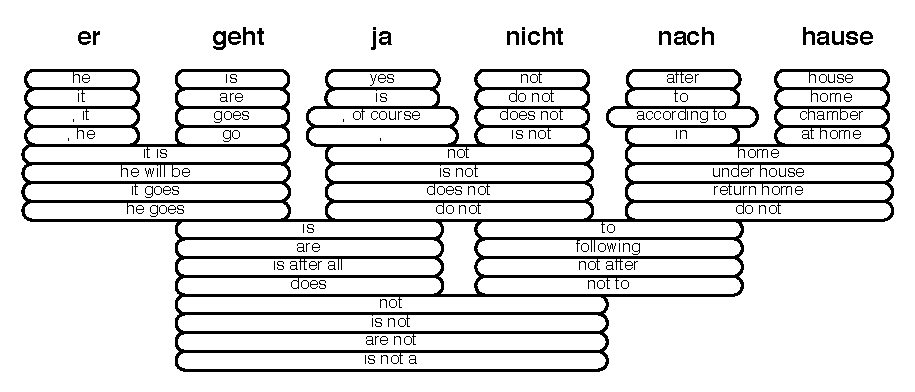
\includegraphics{g/translation-options.pdf}
 \caption{Translation Options}
 \caption*{\textit{\cite{Koehn2009a}}}
\end{figure}

This translation options are used as building blocks in a process known as \textit{hypothesis expansion}. During this process, a data structure known as \textit{search graph} is being built by sequentially joining translation options that cover different parts of sentence in source language (Figure 2.2). Nodes of this graph are called \textit{hypotheses}. As new translation options are being added to existing hypotheses, new partial translation is formed \citep{Koehn2009a}. This process continues until the sequence of hypotheses covers all parts of the input sentence. Each hypothesis contains information about the translation being attached in the current step, the total score of the current partial translation, a link to the previous hypothesis that is extended by the current one and change in the coverage vector of the foreign language sentence.

\begin{figure}
 \centering 
 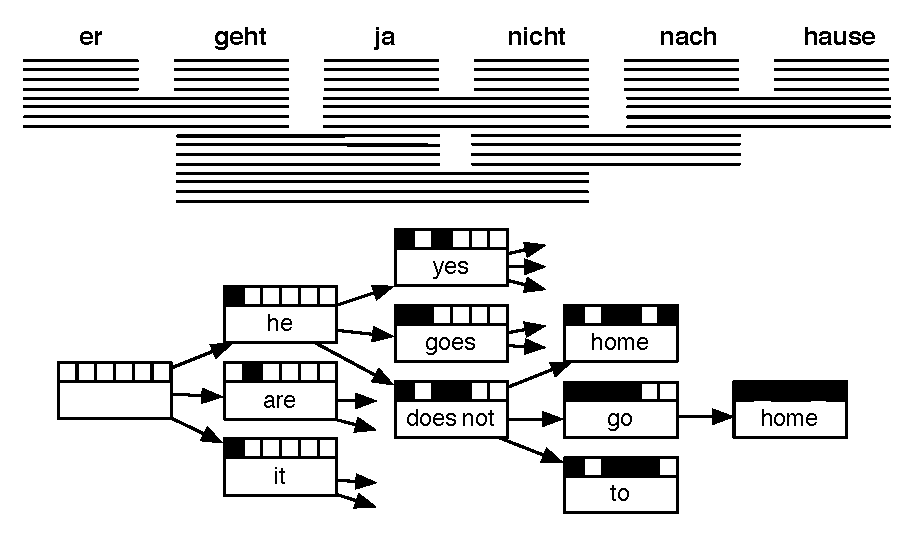
\includegraphics{g/decoding-step5.pdf}
 \caption{Hypothesis expansion}
 \caption*{\textit{\cite{Koehn2009a}}}
\end{figure}

\subsection{Hypothesis recombination}

The resulting data structure is still too large to be directly used for translation search. Several techniques are applied in order to reduce its size. One way is using \emph{hypothesis recombination}, which merges paths with same output and foreign language coverage. This reduction is risk-free and may not cause losing a good translation option. Sample recombination is illustrated on Figures 2.3 and 2.4. Both hypotheses before recombination produce the same output and cover same parts of source sentence, therefore the one with lower score could be recombined to reduce search space. Although this technique removes many unnecessary paths from graph, applying recombination does not affect overall exponential growth in number of hypothesis. 

\begin{figure}
 \centering 
 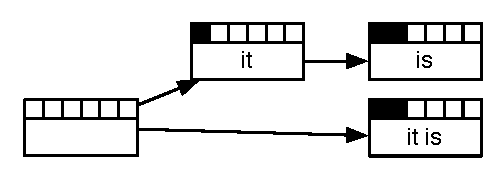
\includegraphics{g/recombination-example1.pdf}
 \caption{Before recombination}
 \caption*{\textit{\cite{Koehn2009a}}}
\end{figure}


\begin{figure}
 \centering 
 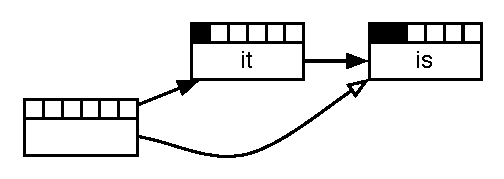
\includegraphics{g/recombination-example2.pdf}
 \caption{After recombination}
 \caption*{\textit{\cite{Koehn2009a}}}
\end{figure}


\subsection{Pruning}

Further reduction of the search graph is required for longer sentences. \textit{Stack decoding} is applied in order to filter hypothesis that have low probability of leading to good translations. Essential difference from recombination is that, this reduction technique is not risk-free and potentially may eliminate some useful translations. During this process stacks containing hypotheses with same coverage are constructed and pruning methods like histogram and threshold pruning are applied. As result number of items in stacks are reduced. 

\subsection{Summary}

In this section we provided a brief introduction into phrase-based Statistical Machine Translation, focusing on decoding stage during which search graph is being produced. Two reasons of erroneous translation produced by the process we described are \textit{search error} and \textit{model error}. While the first one corresponds to failure of finding the highest scoring translation during search, the second one refers to initial problems in the machine translation model. The assistance tool developed and investigated by us aims to help users to fix these errors within a Computer Aided Translation system by pointing to erroneous parts and selecting a better paraphrasing option from the suggestions list. In some sense our approach lets user reuse information collected during decoding. This information is available as search graph output, which optionally could be returned by Moses, together with translation results. 

%% ... etc ...

%%%%%%%%
%% Any appendices should go here. The appendix files should look just like the
%% chapter files.
\appendix
\include{appendix1}
%% ... etc...

%% Choose your favourite bibliography style here.
\bibliographystyle{apalike}

%% If you want the bibliography single-spaced (which is allowed), uncomment
%% the next line.
% \singlespace

%% Specify the bibliography file. Default is thesis.bib.
\bibliography{thesis}

%% ... that's all, folks!
\end{document}
